% !TEX program = xelatex
\documentclass[10pt,letterpaper,twocolumn]{article}

% === GEOMETRY ===
\usepackage[top=0.75in, bottom=0.75in, left=0.75in, right=0.75in]{geometry}

% === FONTS ===
\usepackage{fontspec}
\usepackage{unicode-math}
\usepackage{xeCJK}
\setCJKmainfont{Droid Sans Fallback}

\setmainfont{Latin Modern Roman}
\setsansfont{Latin Modern Sans}

\newfontfamily\acbold{ywft-processing-bold}[
  Path=../../system/public/type/webfonts/,
  Extension=.ttf
]
\newfontfamily\aclight{ywft-processing-light}[
  Path=../../system/public/type/webfonts/,
  Extension=.ttf
]
\newfontfamily\kidlispfont{ComicRelief-Regular}[
  Path=fonts/,
  Extension=.ttf
]
\newfontfamily\kidlispbold{ComicRelief-Bold}[
  Path=fonts/,
  Extension=.ttf
]
\setmonofont{Latin Modern Mono}[Scale=0.85]

% === PACKAGES ===
\usepackage{xcolor}
\usepackage{titlesec}
\usepackage{enumitem}
\usepackage{booktabs}
\usepackage{tabularx}
\usepackage{multicol}
\usepackage{fancyhdr}
\usepackage{hyperref}
\usepackage{graphicx}
\graphicspath{{figures/}}
\usepackage{ragged2e}
\usepackage{listings}
\usepackage{natbib}
\usepackage[colorspec=0.92]{draftwatermark}

% === COLORS (AC palette) ===
\definecolor{acpink}{RGB}{180,72,135}
\definecolor{acpurple}{RGB}{120,80,180}
\definecolor{acdark}{RGB}{64,56,74}
\definecolor{acgray}{RGB}{119,119,119}
\definecolor{klbrand}{RGB}{205,92,155}
\definecolor{klcyan}{RGB}{112,214,255}
\definecolor{kldark}{RGB}{48,43,58}
\definecolor{draftcolor}{RGB}{205,92,155}

% === DRAFT WATERMARK ===
\DraftwatermarkOptions{
  text=WORKING DRAFT,
  fontsize=3cm,
  color=draftcolor!18,
  angle=45,
  pos={0.5\paperwidth, 0.5\paperheight}
}

% === KIDLISP SYNTAX COLORS ===
\definecolor{klfn}{RGB}{0,136,170}
\definecolor{klform}{RGB}{119,51,170}
\definecolor{klrepeat}{RGB}{170,0,170}
\definecolor{klnum}{RGB}{204,0,102}
\definecolor{klstr}{RGB}{170,120,0}
\definecolor{klcmt}{RGB}{102,102,102}
\definecolor{klmath}{RGB}{0,136,0}
\definecolor{klvar}{RGB}{204,102,0}
\definecolor{klembed}{RGB}{0,136,0}

\newcommand{\kn}[1]{\textcolor{klnum}{#1}}
\newcommand{\kt}[1]{\textcolor{klstr}{#1}}
\newcommand{\kv}[1]{\textcolor{klvar}{#1}}
\newcommand{\ke}[1]{\textcolor{klembed}{\textbf{#1}}}
\newcommand{\km}[1]{\textcolor{klmath}{#1}}

% === HYPERREF ===
\hypersetup{
  colorlinks=true,
  linkcolor=acpurple,
  urlcolor=acpurple,
  citecolor=acpurple,
  pdfauthor={Jeffrey Alan Scudder},
  pdftitle={KidLisp '26：面向生成艺术的极简Lisp},
}

% === SECTION FORMATTING ===
\titleformat{\section}
  {\normalfont\bfseries\normalsize\uppercase}
  {\thesection.}
  {0.5em}
  {}
\titlespacing{\section}{0pt}{1.2em}{0.3em}

\titleformat{\subsection}
  {\normalfont\bfseries\small}
  {\thesubsection}
  {0.5em}
  {}
\titlespacing{\subsection}{0pt}{0.8em}{0.2em}

% === HEADER/FOOTER ===
\pagestyle{fancy}
\fancyhf{}
\renewcommand{\headrulewidth}{0pt}
\fancyhead[C]{\footnotesize\color{acpink}\textit{工作草稿 --- 请勿引用}}
\fancyfoot[C]{\footnotesize\thepage}

% === CUSTOM COMMANDS ===
\newcommand{\acdot}{{\color{acpink}.}}
\newcommand{\kidlisp}{\textsc{KidLisp}}

% === LISTINGS ===
\lstdefinelanguage{kidlisp}{
  morekeywords=[1]{wipe,ink,line,box,circle,tri,plot,flood,shape,zoom,scroll,spin,blur,contrast,embed,layer,width,height,frame,time,wiggle,melody,mic,suck,sort,form,trans,cube,move,scale,hop,overtone,resolution,write,text,type,stamp,paste,point,poly,noise,fade,pan,unpan,mask,unmask,flip},
  morekeywords=[2]{def,let,if,cond,once,later,lambda,do},
  morekeywords=[3]{repeat},
  morekeywords=[4]{random,sin,cos,tan,floor,ceil,round,abs,sqrt,min,max},
  sensitive=true,
  morecomment=[l]{;},
  morestring=[b]",
  escapeinside={|}{|},
}
\lstset{
  language=kidlisp,
  basicstyle=\ttfamily\small,
  keywordstyle=[1]\color{klfn}\bfseries,
  keywordstyle=[2]\color{klform}\bfseries,
  keywordstyle=[3]\color{klrepeat}\bfseries,
  keywordstyle=[4]\color{klmath},
  commentstyle=\color{klcmt}\itshape,
  stringstyle=\color{klstr},
  breaklines=true,
  frame=single,
  rulecolor=\color{acgray!30},
  backgroundcolor=\color{acgray!5},
  xleftmargin=0.5em,
  xrightmargin=0.5em,
  aboveskip=0.5em,
  belowskip=0.5em,
}

\lstdefinelanguage{json}{
  basicstyle=\ttfamily\small,
  stringstyle=\color{acpink},
  morestring=[b]",
  literate=
    {:}{{{\color{acgray}:}}}{1}
    {,}{{{\color{acgray},}}}{1}
    {\{}{{{\color{acgray}\{}}}{1}
    {\}}{{{\color{acgray}\}}}}{1},
}

% === LIST SETTINGS ===
\setlist[itemize]{nosep, leftmargin=1.2em, itemsep=0.1em}
\setlist[enumerate]{nosep, leftmargin=1.2em}

\setlength{\columnsep}{1.8em}
\setlength{\parindent}{1em}
\setlength{\parskip}{0.3em}

% Hyphenation for narrow two-column layout
\tolerance=800
\emergencystretch=1em
\hyphenpenalty=50

\begin{document}

\twocolumn[{%
\begin{center}

\includegraphics[height=4em]{pals}\par\vspace{0.5em}
{\kidlispbold\fontsize{26pt}{30pt}\selectfont\color{kldark} Kid{\color{klbrand}Lisp} '26}\par
\vspace{0.2em}
{\kidlispfont\fontsize{11pt}{13pt}\selectfont\color{klbrand} 面向生成艺术的极简Lisp}\par
\vspace{0.6em}
{\normalsize Jeffrey Alan Scudder}\par
{\small\color{acgray} Aesthetic Inc.}\par
{\small\color{acgray} ORCID: \href{https://orcid.org/0009-0007-4460-4913}{0009-0007-4460-4913}}\par
\vspace{0.3em}
{\small\color{acpurple} \url{https://kidlisp.com} \enspace$\cdot$\enspace \url{https://aesthetic.computer}}\par
\vspace{0.6em}
\rule{\textwidth}{1.5pt}
\vspace{0.5em}
\end{center}

\begin{center}
{\small\color{acpink}\textbf{[ 工作草稿 --- 请勿引用 ]}}
\end{center}
\vspace{0.3em}

\begin{quote}
\small\noindent\textbf{摘要。}
\kidlisp{}是一种面向生成艺术和交互视听体验的极简Lisp方言。它运行在Aesthetic Computer——一个基于浏览器的创意计算平台——内部。程序存储在MongoDB中，分配简短的字母数字代码，并可通过URL执行。一个15,000行的树遍历求值器提供118个内置函数，涵盖绘图、颜色、变换、数学、动画和音频——没有文件I/O、网络或通用字符串操作——使得任意用户提交的代码可以安全执行。本文描述了语言设计、存储与分发基础设施、媒体流水线，并报告了59位作者创建超过16,000个程序的采用情况。我们论证，将社交分发直接嵌入领域特定语言——而非附加其上——会产生质的不同的创意编程实践。
\end{quote}
\vspace{0.5em}
}]

\section{引言}

创意编程环境通常要求用户在产生视觉或声音输出之前学习一种通用编程语言。Processing~\citep{reas2007processing}使用Java；p5.js~\citep{mccarthy2015p5js}使用JavaScript；Sonic Pi~\citep{aaron2016sonic}使用类Ruby结构。虽然这些工具极大地降低了计算表达的门槛，但它们仍然需要对变量、函数、控制流的熟悉——在许多情况下——还需要本地开发环境。

\kidlisp{}从一个不同的问题出发：\emph{能够产生有趣生成艺术的最小语言是什么？}答案是一个具有精心选择的内置函数、没有用户定义过程、以及不需要安装的浏览器原生运行时的Lisp。一个完整的动画程序可以是一行：

\begin{lstlisting}
(ink |\kt{rainbow}|) (repeat |\kn{100}| |\kv{i}|
  (circle (wiggle width) (wiggle height) |\kn{10}|))
\end{lstlisting}

该设计源于No Paint（2020）的观察——这是一个像素画工具，其非技术用户社区证明了人们通过对其热爱的软件的社交参与来学习计算。\kidlisp{}将这一洞察扩展到编程语言：每个程序都可以通过短代码即时分享，在URL上查看，并嵌入到其他程序中。

本文描述了语言设计（\S\ref{sec:design}）、求值器架构（\S\ref{sec:architecture}）、存储与分发基础设施（\S\ref{sec:infrastructure}）、媒体流水线（\S\ref{sec:media}）以及采用数据（\S\ref{sec:evaluation}）。

\begin{figure}[t]
\centering
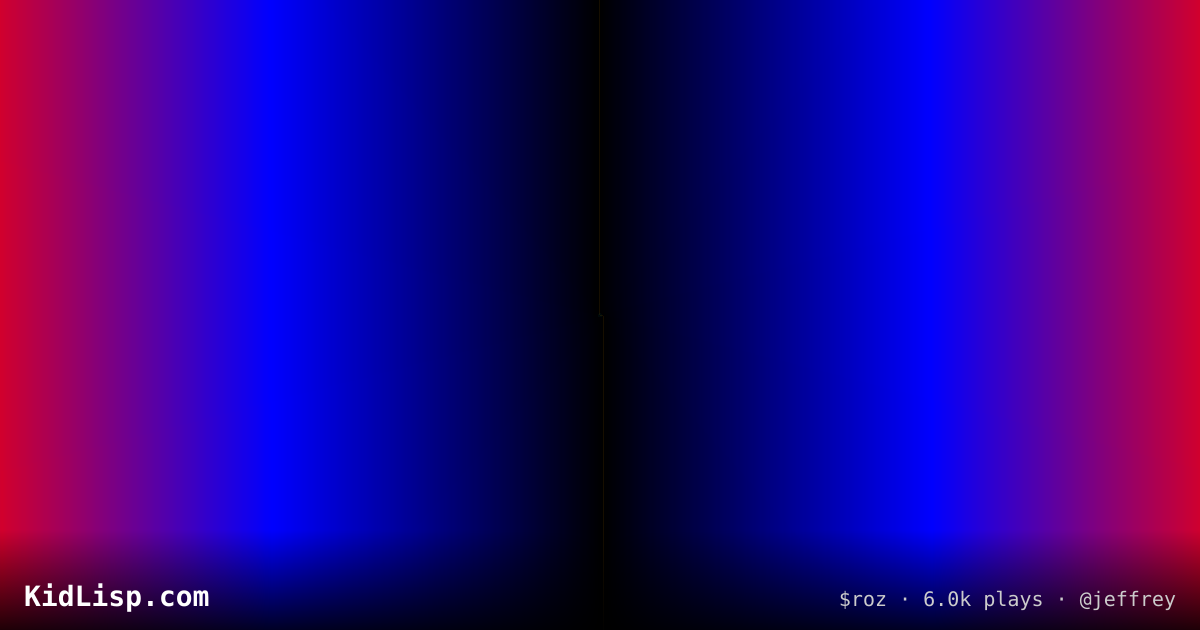
\includegraphics[width=\columnwidth]{kidlisp-og-mosaic.png}
\caption{由oven服务渲染的精选\kidlisp{}程序（\texttt{\$roz}）Open Graph社交预览。叠加层显示程序代码、播放次数和作者标识。}
\label{fig:og}
\end{figure}

\section{语言设计}
\label{sec:design}

\kidlisp{}是一种S表达式语言。每个程序是从上到下求值的表达式序列，在HTML Canvas 2D上下文、WebGL上下文、Web Audio图或其组合上产生副作用。

\subsection{设计原则}

\begin{enumerate}
  \item \textbf{每个表达式都会绘制。}有效的\kidlisp{}会产生可见输出。没有\texttt{main}，没有导入，没有样板代码。
  \item \textbf{扁平胜于嵌套。}程序通过嵌入其他程序来组合，而非通过定义抽象。这使代码一目了然地可读。
  \item \textbf{构造即安全。}没有文件I/O，没有网络，没有外部状态的修改。程序通过语言缺少危险原语来实现沙箱化。
  \item \textbf{默认社交。}每个程序都有短代码和URL。分享是分发机制，而非事后附加。
\end{enumerate}

\subsection{函数分类}

118个内置函数涵盖12个类别（表~\ref{tab:functions}）。

\begin{table}[h]
\small
\centering
\begin{tabularx}{\columnwidth}{lrX}
\toprule
\textbf{类别} & \textbf{数量} & \textbf{示例} \\
\midrule
图形 & 9 & \texttt{wipe}, \texttt{ink}, \texttt{line}, \texttt{box}, \texttt{circle} \\
变换 & 11 & \texttt{scroll}, \texttt{zoom}, \texttt{spin}, \texttt{blur}, \texttt{suck} \\
数学 & 14 & \texttt{+}, \texttt{sin}, \texttt{cos}, \texttt{random}, \texttt{wiggle} \\
颜色 & 19 & CSS名称 + \texttt{rainbow}, \texttt{zebra} \\
系统 & 9 & \texttt{width}, \texttt{height}, \texttt{frame}, \texttt{fps} \\
3D & 8 & \texttt{cube}, \texttt{form}, \texttt{trans}, \texttt{move} \\
音频 & 6 & \texttt{mic}, \texttt{melody}, \texttt{overtone} \\
控制 & 7 & \texttt{def}, \texttt{if}, \texttt{repeat}, \texttt{once}, \texttt{later} \\
文本 & 4 & \texttt{write}, \texttt{type}, \texttt{paste} \\
输入 & 3 & \texttt{pen}, \texttt{touch} \\
组合 & 4 & \texttt{embed}, \texttt{layer}, \texttt{fade} \\
数据 & 4 & \texttt{let}, \texttt{list}, \texttt{get}, \texttt{set} \\
\midrule
\textbf{总计} & \textbf{118} & \\
\bottomrule
\end{tabularx}
\caption{按类别分类的内置函数。}
\label{tab:functions}
\end{table}

\begin{figure}[t]
\centering
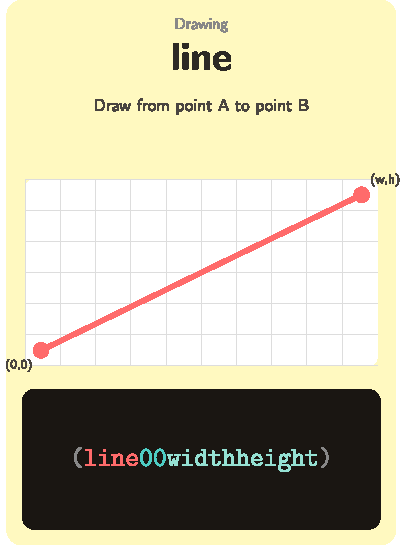
\includegraphics[height=4.5cm]{card-line.pdf}%
\hfill%
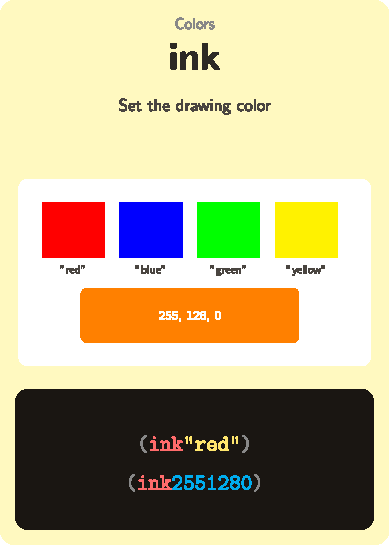
\includegraphics[height=4.5cm]{card-ink.pdf}
\caption{\kidlisp{}\texttt{line}和\texttt{ink}函数的参考卡，显示语法和坐标输出。卡片以SVG插图形式分发于\texttt{kidlisp.com/cards}。}
\label{fig:cards}
\end{figure}

\subsection{时序语法}

\kidlisp{}提供时序运算符，无需显式循环或回调即可调度表达式求值：

\begin{lstlisting}
|\kt{2.5s}| (wipe |\kt{red}|)           ; after 2.5 seconds
|\kt{1s...}| (spin |\kn{5}|)            ; repeat every second
|\kt{3s!}| (write "Done" |\kn{10}| |\kn{10}|)  ; fire exactly once at 3s
|\kt{30f}| (ink |\kt{blue}|)             ; after 30 frames
\end{lstlisting}

后缀\texttt{s}表示秒，\texttt{f}表示帧，\texttt{...}表示重复，\texttt{!}表示单次执行。这些运算符可以组合：\texttt{0.5s... (ink (random 255) (random 255) (random 255))}每半秒产生一次颜色变化。

\subsection{KidLisp省略的内容}

该语言刻意排除了用户定义函数（除了用于命名值的\texttt{def}）、递归、字符串操作、文件I/O、网络、可变数据结构和异常处理。这些省略就是设计本身。通过移除抽象机制，程序保持扁平和可读——读者可以从上到下理解任何程序而无需追踪调用栈。

\section{求值器架构}
\label{sec:architecture}

求值器（\texttt{kidlisp.mjs}，15,161行）是一个单独的JavaScript ES模块，实现了一个树遍历解释器。

\subsection{求值模型}

求值器每个动画帧运行一次。S表达式被标记化并解析为嵌套数组AST，然后通过对每个列表第一个符号的分派进行遍历。内置函数直接映射到Canvas 2D操作、WebGL命令、Web Audio API调用和数学计算。整个程序每帧重新求值，\texttt{frame}和\texttt{time}绑定自动更新——一种消除显式动画循环的即时模式模型。

\subsection{确定性渲染}

给定相同的随机种子和帧数，程序总是产生相同的输出。\texttt{random}函数使用从程序短代码初始化的种子PRNG，实现可复现的生成艺术。

\subsection{混沌模式}

无效或随机文本输入触发艺术性视觉输出而非错误消息。一个基于置信度评分的检测器检查词语识别率（$<$30\%已知词汇）、特殊字符比率（$>$50\%）和括号平衡（比率$>$3:1）来将输入分类为代码或混沌。混沌输入产生从输入文本种子生成的确定性生成视觉效果。这意味着输入到\kidlisp{}中的\emph{任何}文本都会产生视觉内容——用户不会看到任何错误状态。

\subsection{性能}

求值器实现了三个优化级别：

\begin{itemize}
  \item \textbf{多级代码缓存}：嵌入程序解析依次检查RAM、IndexedDB、网络，然后TEIA（去中心化存档）。缓存命中避免重新解析和重新获取。
  \item \textbf{缓冲区池化}：每个分辨率最多8个可复用的离屏画布，避免合成期间的分配抖动。
  \item \textbf{自动密度缩放}：像素密度基于滚动FPS平均值（目标：30--55 FPS）在0.5x和4x之间调整，调整间有60帧冷却时间。
\end{itemize}

函数调用结果、alpha调整的像素缓冲区和混合合成体逐帧缓存和失效。

\section{存储与分发}
\label{sec:infrastructure}

\subsection{MongoDB存储}

每个程序作为\texttt{kidlisp} MongoDB集合中的文档存储：

\begin{lstlisting}[language=json]
{
  "code": "cow",
  "source": "(wipe blue)\n(ink yellow)...",
  "hash": "a3f2e8...",
  "when": "2025-06-15T...",
  "lastAccessed": "2026-03-01T...",
  "hits": 342,
  "user": "auth0|abc123"
}
\end{lstlisting}

\texttt{hash}字段（修剪后源码的SHA-256）强制基于内容的去重：相同的程序总是解析为相同的代码。\texttt{hits}计数器和\texttt{lastAccessed}时间戳用于使用分析。集合在\texttt{code}和\texttt{hash}上维护唯一索引，加上\texttt{user}和可选NFT铸造记录（\texttt{kept.network}）上的稀疏索引。

\subsection{代码生成}

短代码由源码感知算法生成。系统首先尝试从程序内容派生有意义的代码——提取主要函数名、颜色关键字或结构模式——如果所有推断的代码已被占用则回退到随机\texttt{nanoid}生成。这产生了像\texttt{cow}（一个有牛形状的程序）这样的代码，而非任意的字母数字字符串。

\subsection{REST API}

存储端点（\texttt{store-kidlisp.mjs}）在单一URL上提供五种查询模式：

\begin{enumerate}
  \item \textbf{POST} --- 存储程序。通过SHA-256哈希去重，生成短代码，可选同步到ATProto（Bluesky）并发布档案事件。
  \item \textbf{GET \texttt{?code=xyz}} --- 检索单个程序，通过\texttt{\$lookup}在\texttt{@handles}集合上解析作者标识。
  \item \textbf{GET \texttt{?codes=a,b,c}} --- 批量检索（最多50个代码），用于求值期间的嵌入层解析。
  \item \textbf{GET \texttt{?recent=true}} --- 按创建时间或点击量排序的分页feed，可选\texttt{handle}过滤器用于按用户的feed。
  \item \textbf{GET \texttt{?stats=functions}} --- 跨语料库的函数使用分析，返回按程序人气加权的计数。
\end{enumerate}

认证可选且有3秒超时——支持匿名程序创建，但认证用户获得归属和档案事件发布。

\subsection{嵌入与组合}

程序内的\texttt{\$code}语法触发从存储API获取（或缓存命中）、在离屏缓冲区中求值，并合成到父画布上。这创建了一个有向无环组合图。一个实际例子：

\begin{lstlisting}
; A 3D grid of cubes with embedded layers
(wipe |\kt{black}|)
(def |\kv{gridsize}| |\kn{6}|)
(repeat (|\km{*}| |\kv{gridsize}| |\kv{gridsize}|) |\kv{i}|
  (ink (hop |\kn{0.1}| |\kt{rainbow}| |\kt{blue}| |\kt{white}|))
  (form (trans (cube |\kv{i}|)
    (move (|\km{*}| (|\km{\%}| |\kv{i}| |\kv{gridsize}|) |\kn{3}|) |\kn{0}| |\kn{-20}|)
    (scale |\kn{1.5}|) (spin |\kn{0}| |\kn{1}| |\kn{0}|))))
(|\ke{\$27z}|)
(|\ke{\$cow}|)
\end{lstlisting}

这里\texttt{\$27z}和\texttt{\$cow}从MongoDB解析，渲染到离屏缓冲区中，并合成。用户通过叠加简单程序而非编写复杂的单一程序来构建复杂的视觉效果。

\section{媒体流水线}
\label{sec:media}

oven服务（\texttt{oven.aesthetic.computer}）将录制的\kidlisp{}会话转换为可分享的媒体资产。

\subsection{录制转MP4}

当用户录制会话时，会话服务器上传包含PNG帧和可选WAV音频的ZIP。oven：

\begin{enumerate}
  \item 提取帧并读取\texttt{timing.json}获取每帧持续时间
  \item 从中间帧生成缩略图（3倍最近邻放大，适配512$\times$512）
  \item 通过FFmpeg使用最近邻放大编码为H.264/AAC MP4以保持像素画美感
  \item 上传到DigitalOcean Spaces CDN
  \item 在\texttt{oven-bakes} MongoDB集合中存储烘焙元数据，并通过WebSocket通知订阅者
\end{enumerate}

oven通过变更流监视\texttt{tapes} MongoDB集合，自动检测需要处理的新录制。

\begin{figure}[t]
\centering
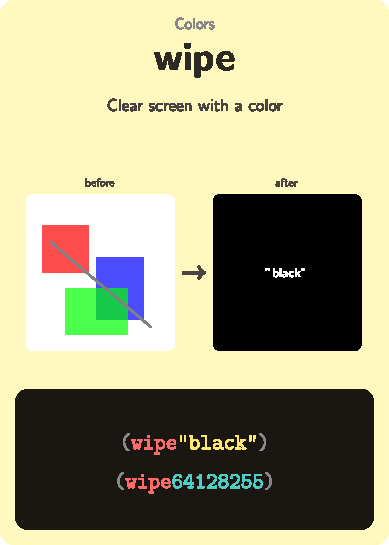
\includegraphics[height=4.5cm]{card-wipe.pdf}%
\hfill%
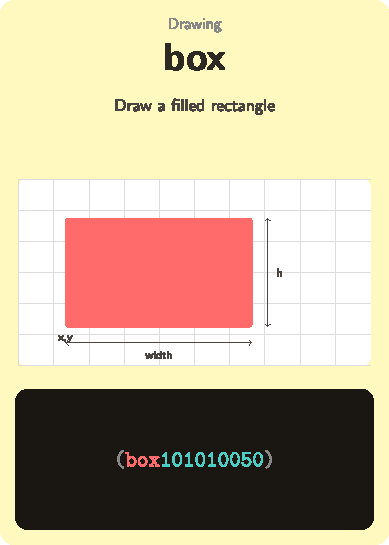
\includegraphics[height=4.5cm]{card-box.pdf}
\caption{\texttt{wipe}（用颜色清除屏幕）和\texttt{box}（绘制矩形）的参考卡。每张卡显示函数签名、网格上的视觉示例和对应的源代码。}
\label{fig:cards2}
\end{figure}

\subsection{社交预览图片}

oven为社交分享生成稳定URL（例如\texttt{/kidlisp-og.png}）的Open Graph预览图片。iOS爬虫要求直接图片服务——它们不会跟随\texttt{og:image} URL上的301重定向——因此oven缓存生成的PNG并以即时200响应服务，在缓存未命中时触发异步重新生成。

\subsection{资产交付}

所有媒体资产通过DigitalOcean Spaces CDN（\texttt{art-aesthetic-computer.sfo3.cdn.\allowbreak digitaloceanspaces.com}）提供服务。录制磁带使用单独的存储桶（\texttt{at-blobs-aesthetic-computer}）和可选的自定义CDN域名。Netlify代理\texttt{/preview/*}和\texttt{/icon/*}路径到oven以实现透明URL解析。

\section{开发环境}

\kidlisp{} IDE位于\texttt{kidlisp.com}，提供基于Monaco的编辑器（具有自定义语法高亮）、运行Aesthetic Computer运行时的实时预览iframe、控制台面板和播放控件（播放/暂停/停止）。

"滑块模式"允许拖动编辑器中的数字字面量实时调整值——光标在任何数字上变为水平滑块，拖动期间预览持续更新。

IDE支持两种布局模式：\emph{工作室}（分屏编辑器、预览和控制台）和\emph{舞台}（编辑器直接覆盖在全屏画布上，透明背景，所有界面元素隐藏）。舞台模式设计用于现场表演场景，代码本身成为视觉输出的一部分。

\section{开发历史}
\label{sec:history}

以下时间线根据Aesthetic Computer仓库的git历史重建（2024年4月至2026年3月间触及\texttt{kidlisp.mjs}的626次提交）。

\subsection{第一阶段：原型（2024年4--6月）}

开发始于2024年4月17日，提交标题为"mock lisp"。三天内，S表达式解析器已经工作，\texttt{ink}和\texttt{line}接受数字参数，程序可以直接在AC提示符中输入。4月末，添加了\texttt{def}用于变量定义。2024年5月和6月共66次提交，添加了核心绘图函数、\texttt{later}时序结构、用于一次性执行的\texttt{once}，以及程序的匿名发布。求值器达到约1,000行。

\subsection{第二阶段：停滞（2024年7月--2025年5月）}

11个月内没有提交触及\texttt{kidlisp.mjs}。该语言作为嵌入AC提示符中的可用原型存在，但缺少存储后端、嵌入、音频或专用编辑器。

\subsection{第三阶段：快速扩展（2025年6--8月）}

开发于2025年6月恢复，当月82次提交。求值器从1,760行增长到8月的4,965行。主要新增：

\begin{itemize}
  \item \textbf{2025年6月}：旋律解析器、时钟语法、逐帧渲染模型、测试套件（\texttt{kidlisp-spec.js}）。
  \item \textbf{2025年7月}：MongoDB存储后端（\texttt{store-kidlisp.mjs}）、短代码生成、二维码分享、录制和GIF导出、麦克风输入（\texttt{mic}）带回退动画。
  \item \textbf{2025年8月}：嵌入层（\texttt{\$code}语法）带alpha合成和离屏缓冲、Tezos区块链集成用于将程序铸造为NFT、\texttt{fade}渐变和像素缓冲区优化。
\end{itemize}

求值器在2025年9月末超过10,000行。

\subsection{第四阶段：平台整合（2025年9--12月）}

仅10月就有108次提交（峰值月），此阶段将\kidlisp{}整合到更广泛的Aesthetic Computer生态系统中：

\begin{itemize}
  \item \textbf{2025年9月}：第0层架构（擦除模式）、MP4导出的烘焙分层、性能关键的嵌入层修复。
  \item \textbf{2025年10月}：ATProto/Bluesky联合（程序作为社交媒体帖子联合发布）、PACK模式用于跨平台捆绑、滑块模式用于实时数字参数调整。
  \item \textbf{2025年11月}：\texttt{kidlisp.com} IDE上线（Monaco编辑器、实时预览、控制台、播放控件）、调试用执行跟踪系统、NFT工作流从"OBJKT"重命名为"keep"。
  \item \textbf{2025年12月}：参考卡（每个函数的SVG插图）、NFT的IPFS缩略图生成、社交分享的oven OG图片生成、自动密度性能缩放。
\end{itemize}

\subsection{第五阶段：完善（2026年1--3月）}

求值器稳定在15,161行。新增包括混沌模式（2026年2月）、3D原语（\texttt{cube}、\texttt{form}、\texttt{trans}）、频段音频变量、\texttt{flip}命令和用于现场表演的舞台模式。开发从功能添加转向健壮性：修复嵌入层性能回归、防止混沌模式误分类、改善缓存失效。

\begin{table}[h]
\small
\centering
\begin{tabular}{lrl}
\toprule
\textbf{日期} & \textbf{行数} & \textbf{里程碑} \\
\midrule
2024年4月 & 0 & 初始提交（"mock lisp"） \\
2024年6月 & $\sim$1{,}000 & 核心绘图、时序、变量 \\
2025年6月 & 1{,}760 & 开发恢复 \\
2025年8月 & 4{,}965 & 嵌入、音频、存储 \\
2025年9月 & 10{,}382 & 层架构、烘焙 \\
2025年12月 & 13{,}877 & IDE、卡片、OG图片 \\
2026年2月 & 15{,}161 & 混沌模式、3D、完善 \\
\bottomrule
\end{tabular}
\caption{求值器按行数增长（\texttt{kidlisp.mjs}）。}
\label{tab:growth}
\end{table}

\section{评估}
\label{sec:evaluation}

截至2026年3月的采用指标如表~\ref{tab:adoption}所示。

\begin{table}[h]
\small
\centering
\begin{tabular}{lr}
\toprule
\textbf{指标} & \textbf{数值} \\
\midrule
创建的总程序数 & 16,174 \\
独立作者 & 59 \\
每位作者程序数（中位数） & 12 \\
每位作者程序数（上四分位） & 180+ \\
嵌入深度（观察到的最大值） & 7层 \\
平台注册用户 & 2,798 \\
\bottomrule
\end{tabular}
\caption{采用指标（2026年3月）。}
\label{tab:adoption}
\end{table}

\subsection{函数使用分析}

\texttt{?stats=functions} API端点提供跨语料库的加权函数使用计数。它扫描最多5,000个程序（按点击量排序），解析每个源码以提取函数调用，并返回按程序人气加权的计数。这使得对用户偏好的原语进行定量分析成为可能。最常用的函数是\texttt{wipe}、\texttt{ink}、\texttt{repeat}和\texttt{circle}——确认用户主要使用绘图和迭代。

\subsection{观察}

\textbf{组合胜于抽象。}用户嵌入而非抽象。被引用最多的程序是简单的视觉原语（渐变、形状、图案），充当构建块。

\textbf{探索胜于工程。}程序通常很短（10行以下）。用户通过保存新程序而非编辑现有程序来迭代，在存储时间戳中创造可见的发散探索路径。

\textbf{社交学习。}最多产的作者始于查看和混搭现有程序。短代码系统使发现变得偶然——用户通过尝试随机代码来遇到程序。

\subsection{局限性}

\kidlisp{}不适用于通用编程、复杂模拟或需要跨会话持久化状态的应用。用户定义函数的缺失限制了程序复杂性——这是一个刻意的选择，但一些高级用户对此感到沮丧。

\section{相关工作}

\textbf{创意编程。}Processing~\citep{reas2007processing}和p5.js~\citep{mccarthy2015p5js}是主流工具。openFrameworks使用C++。所有这些都需要管理项目结构并理解通用编程语言。

\textbf{实时编程。}Hydra~\citep{hydra2019}提供基于浏览器的实时视觉编程，使用JavaScript方法链但没有持久存储或社交功能。Sonic Pi~\citep{aaron2016sonic}面向音乐教育。Fluxus~\citep{fluxus2007}使用Scheme进行3D视觉效果但已不再维护。

\textbf{教育语言。}Scratch~\citep{resnick2009scratch}证明了社交分享推动教育编程的参与度。\kidlisp{}继承了这一洞察，但使用基于文本的Lisp语法，面向生成艺术而非通用教育。

\textbf{艺术用Lisp。}Racket的\texttt{2htdp/image}库~\citep{racket2018}为CS教育提供函数式图像构建，但面向静态图像和教学法，而非带有社交分发的实时动画。

\section{结论}

\kidlisp{}证明了一种极简领域特定语言——浏览器原生、没有用户定义的抽象、由带有社交分发的内容寻址数据库支持——可以支持一个活跃的生成艺术实践社区。关键的设计洞察是，社交分发（短代码、URL分享、嵌入）不是附加功能而是核心语言特性，塑造了用户如何学习、创作和在彼此工作基础上构建。

嵌入图、函数使用分析API以及16,000+个带有时间戳和作者归属的程序语料库构成了研究创意编程实践、计算创造力以及非专家用户如何通过社交参与学习函数式编程的数据集。

\kidlisp{}在ISC许可证下开源。求值器、文档和工具可在\url{https://github.com/digitpain/aesthetic.computer}获取。程序可在\url{https://kidlisp.com}浏览和创建。

\vspace{0.5em}
\noindent\textit{翻译自英文原版。原版请访问 \url{https://papers.aesthetic.computer}}

\vspace{0.5em}
\noindent\textbf{ORCID:} \href{https://orcid.org/0009-0007-4460-4913}{0009-0007-4460-4913}

\bibliographystyle{plainnat}
\bibliography{references}

\end{document}
